\chapter{Charaktere}

Im folgenden die wichtigsten Charaktere mit denen es die Spieler zu tun bekommen aufgeteilt nach Ort des Geschehens.

\section{Cowboybrigade}

Die Cowboybrigade sind 5 Alphas, Spezialisten f"ur Raumschifftechnik, Arbeit mit Exoskelett im Luftlehren Raum, Drohneneinsatz.
Angestellt bis vor 6 Wochen am Raumhafen von Valhalla auf Callisto. Dann ausgeliehen an die Protektoratsgarnison am Raumhafen von Valhalla und vor ca.~4 Wochen ausgeliehen an Armageddon. Die Cowboybrigade stammt urspr"nglich aus dem Asteroideng"urtel G"urtel zwischen Mars und Jupiter und ist vor wahrscheinlich einem Jahr auf Callisto.

\begin{itemize}
    \item Stetson: Der Anf"uhrer, gro\3 und dratig.
    \item Quckfinger Rod: Vorlaut, immer ein Kartenspiel in der Hand.
    \item Joe Rider: Klein, gedrungen, spricht nicht wenn nicht unbedingt n"otig.
    \item Tom Gunslinger: Der Vern"unftige.
    \item Slingshot (Drake): Das "`Nesth"akchen"' der Gruppe. Drake ist der Name unter dem er in nach seinem Attentat 
    auf Armageddon auf Hellgate in Erscheinung tritt.
\end{itemize}

\newpage

\section{Pers"onlichkeiten auf Hellgate}

Auf Hellgate gibt es folgende Pers"onlichkeiten: 

\begin{itemize}
    \item Dr.~Acra Link: Technische Leitung der Hellgate Station
    \item Sina Hendrik: Administrative Leitung der Hellgate Station
    \item Dr.~Petrova: Technische Leitung der F"orderminen
    \item Henk Arongate: Sicherheitschef    
    \item Kriegsmeister Jos\'{e} \frqq{}Toro\flqq{} Alvarez: Norm. Ausbilder der Jagdverb"ande des Protektorats, Kriegsheld.
    \item Arbeiter Mob: Fight +2, Agility +1, Body +3, HP 10, Courage +2
\end{itemize}

\section{Sicherheitspersonal Hellgate}

Neben \emph{Grace Anders} sind folgende Personen des Sicherheitsdienstes relevant:

\begin{itemize}
    \item Henk Arongate: Sicherheitschef    
    \item Karl Sandos: Stationsleiter des St"utzpunkts der Sicherheitskr"afte. Vorgesetzter von Grace Anders.
    \item Luke Dexter: Trupp F"uhrer der Sondereinsatzgruppe f"ur die Befreiung der Geiseln.
    \item Luke Lengdon: Mitarbeiter Sicherheitsdienst. Wird bei der Geiselname auf dem Sicherheitsst"utzpunkt schwer 
    verletzt. Ehemaliger Freund von Grace Anders. Seit 2 Wochen getrennt.
\end{itemize}

\section{Geiselnehmer}

Auf Hellgate treten zwei Geiselnehmer f"ur die Befeiung von Hanibal dem Attent"ater auf den Minnen HeM03 und HeM05 in
Erscheinung:

\begin{description}
    \item[Slingshot(Drake)] Slingshot ist einer der Attent"ater, ein Alpha dessen Gehirn durch eine von der USI kontrollierten 
    KI "ubernommen wurde. Auf Hellgate tritt er nach dem Vorfall auf Armageddon unter dem Namen Drake auf.

    \textbf{Slingshot: Fight +4, Agility +4, Body +2, HP 12\\
    Kampfanzug -6, Railgun vollautomatische Pistle +6}

    \item[Smith Henderson] Smith Henderson ist ein S"oldner der durch die USI Agenten telefonisch angeheuert wurde um 
    zusammen mit Drake Hanibal zu befreien und von der Station zu schaffen.

    \textbf{Smith Henderson: Fight +5, Agility +4, Body +1, HP 10\\
    Kampfanzug Schaden -6, Railgun vollautomatisches Gewehr +6, Vibrokling +3}

    \item[Hanibal] Hanibal ist einer der Minenarbeiter und der Attent"ater auf HeM03 und HeM05. Wie Slingshot 

    \textbf{Hanibal: Fight +2, Agility +1, Body +2, HP 12\\
    Schusssichere Weste -4, Bolter +3}
\end{description}


\newpage
\section{Grace Anders}

Grace Anders ist eine Mitarbeiterin des Sicherheitsdienstes auf Hellgate. Sie wird von Chef Henk Arongate zur Unterst"utung der Charaktere abgestellt. 

\begin{wrapfigure}{l}
    {0.45\textwidth}\fbox{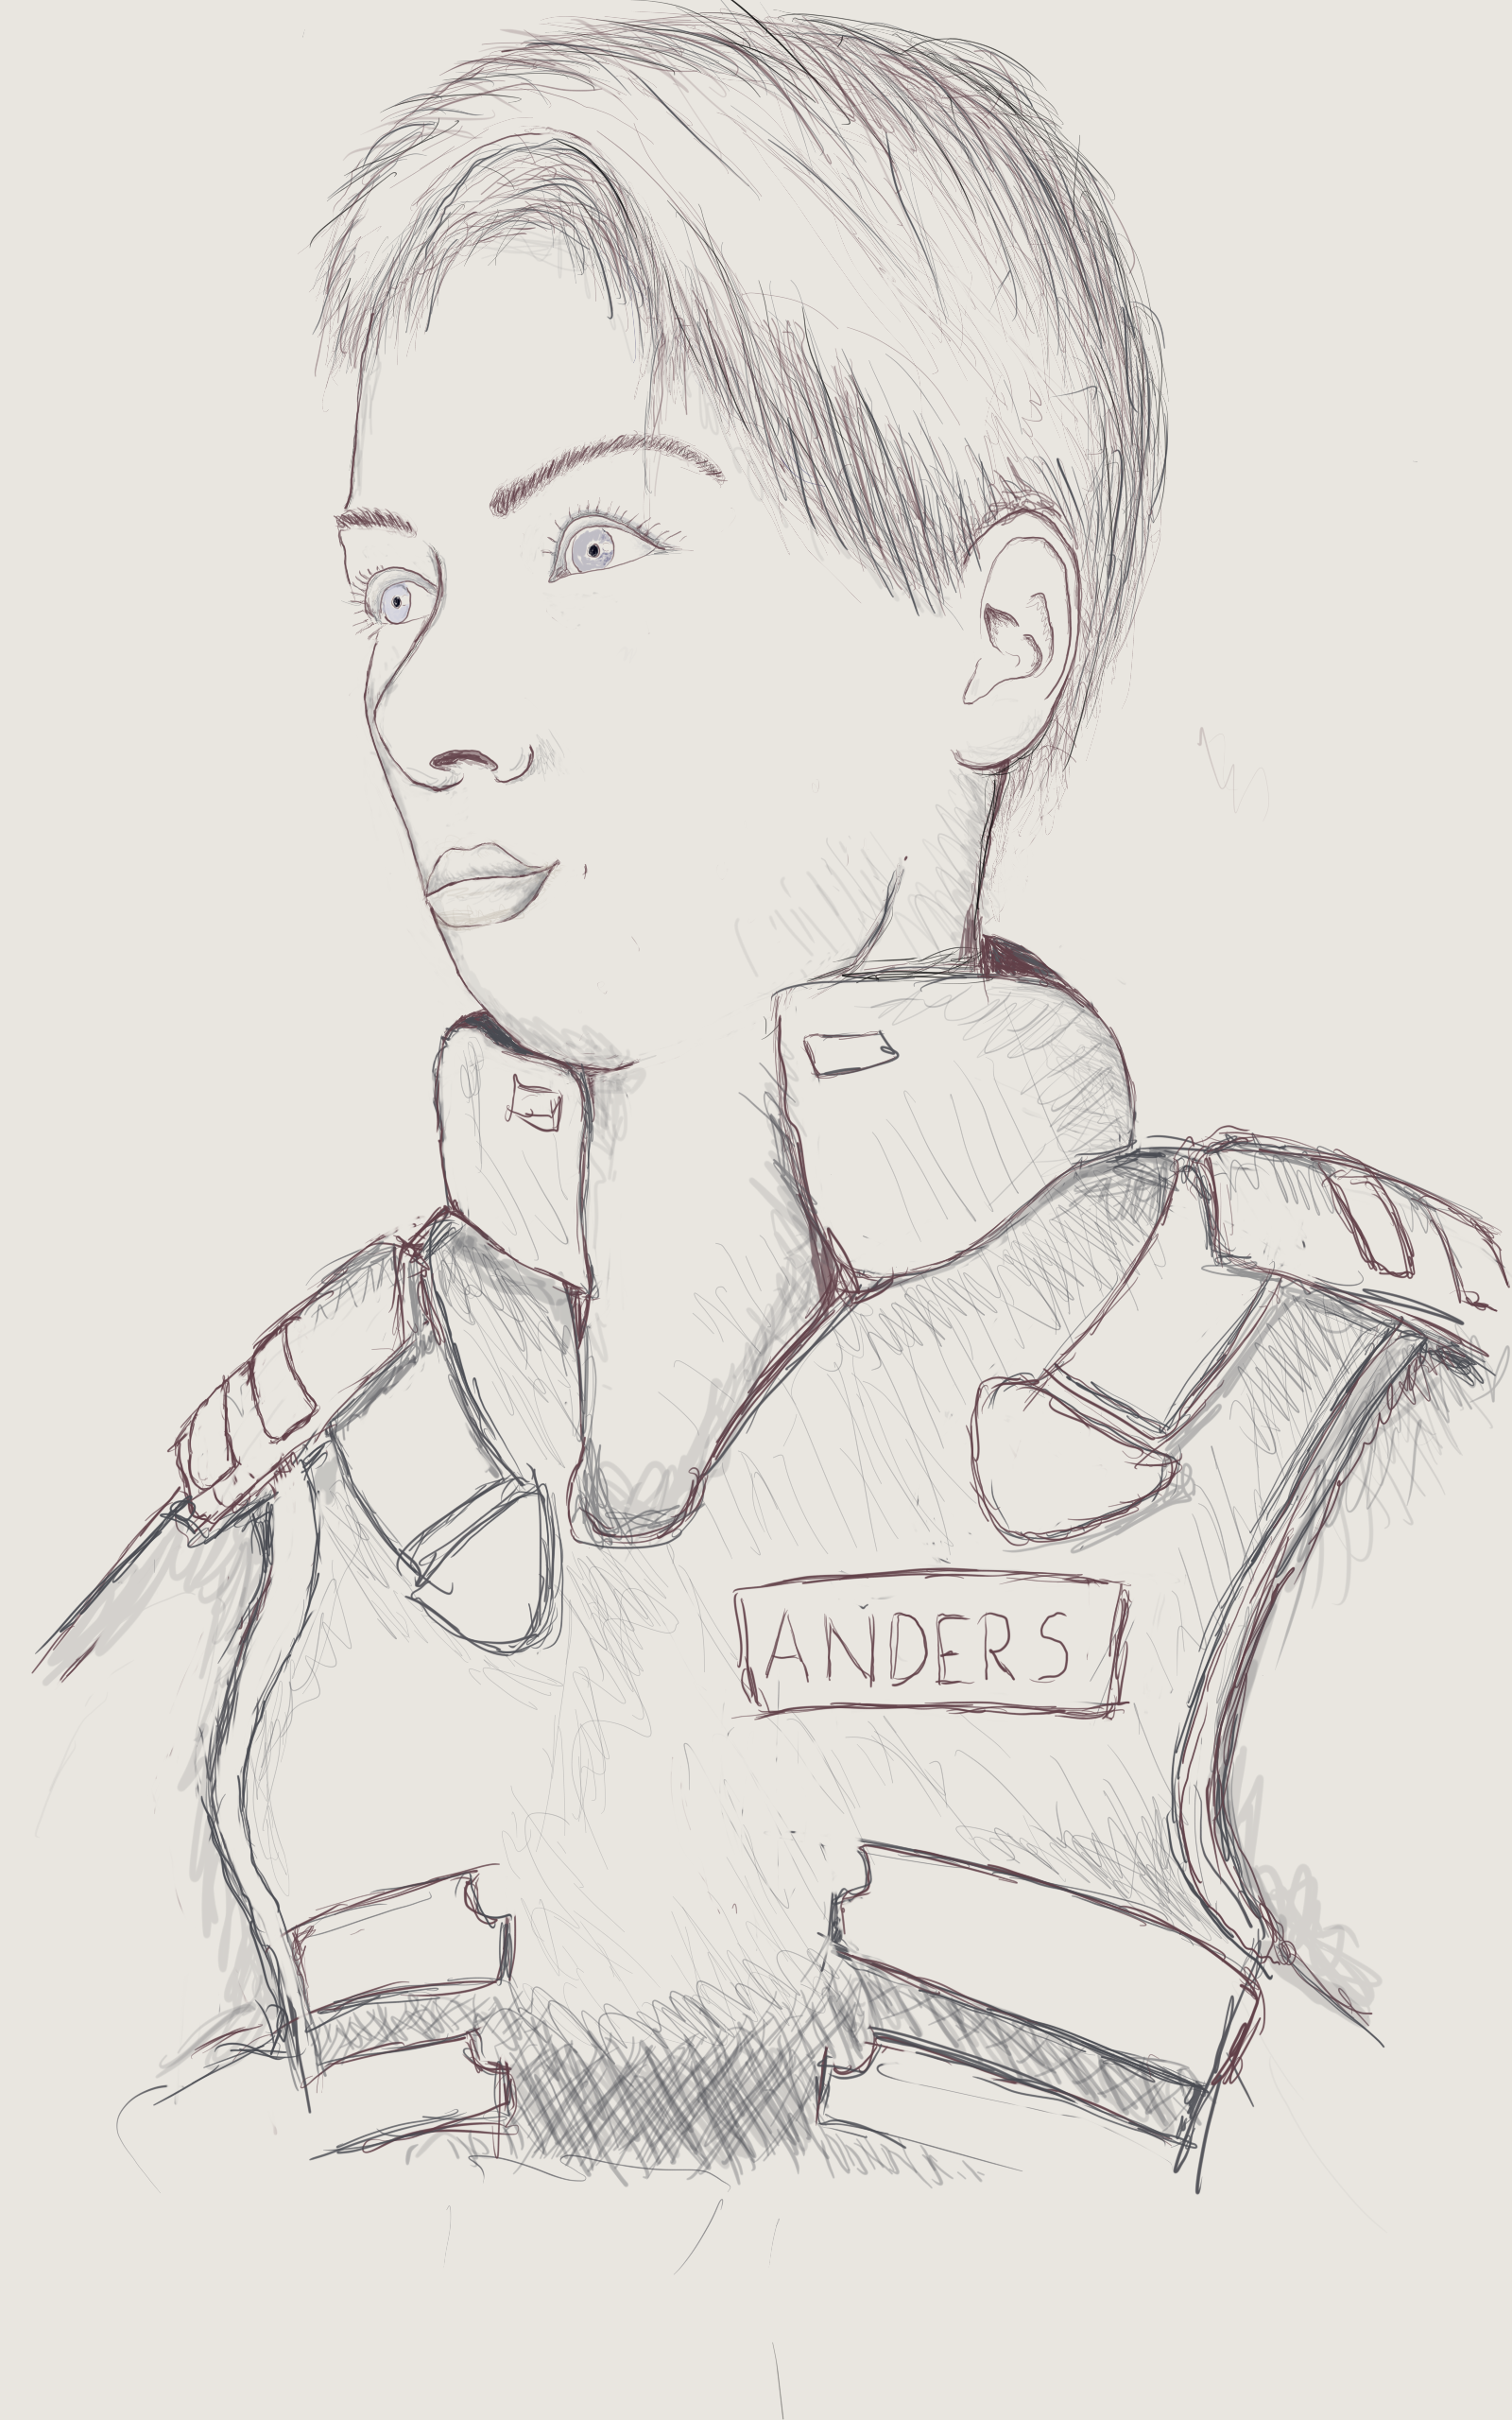
\includegraphics[width=0.90\linewidth]{./images/grace_anders_p.png}}
    \caption{Grace Anders}
\end{wrapfigure}

Grace Anders ist Mitte 30, h"ubsch mit kurzen blonden Haaren. W"ahrend der Unterst"utzung der Charaktere tr"agt sie die Schutzkleidung des Sicherheitsdienstes mit schu\3sicherer Weste, Schlagstock, Handschellen und einer Schu\3waffe. 

Sie stammt urspr"unglich vom Mars und hat sich ins Jovianische System auf der Suche nach neuen Herausforderungen versetzen lassen. Sie war mit Luke Lengdon der Sicherheitsmann bei der folgenden Geiselname schwer verletzt wurde liiert hat sich aber vor kurzem von ihm getrennt.

Die Sicherheitsbeamtin begleitet die Charaketere w"ahrend des aufenthalts auf Hellgate und berichtet regelm"aßig an \emph{Karl Sandos} ihren vorgesetzten. "Uber Grace Anders k"onnen sie Informationen bzgl.~der Minen und Personal der Station und der Mienen anfragen. W"ahrend der Entf"uhrung kann sie die Charaktere unterst"uten.

Grace Anders: Fight +4, Agility +3, Body +2, HP 10

\section{Besatzung HeM05}

Folgende Personen waren w"ahrend des Attentats auf HeM05:

\begin{itemize}
    \item Florence: Beta Mutant, Kommandant der Mine    
    \item ZDee: Alpha Mutant Minenarbeiter (tot)
    \item Greydog: Alpha Mutant, Minenarbeiter
    \item Isabell Sonderleiten: Norm, Chemikerin, Stellvertreterin von Florence
    \item Juri Smirnov: Norm, Logistik
    \item Fernandez Lorend: Norm, Techniker
    \item Hanibal: Alpha Mutant, Techniker der Minensteueranlage, Attent"ater
    \item Pitch: Alpha Mutant, Technikerin der HE-3 der Minensteueranlage
    \item Salvador: Norm, Physiker, Weltraumtechnik
    \item Blackwind: Beta, Sicherheitsdienst
\end{itemize}

All Mitarbeiter auf der Mine au\3er Fernand, Salvador, Greydog und Pitch waren vor dem Jupitereinsatz bereits im Dienst der Cynarion Corporation.

\section{Garnisonsst"utzpunkt Valhalla}

\begin{itemize}
    \item Commander Lockhead ist der Kommandant der Milit"argarnison des Protektorats auf Valhalla. Commander Lockhead ist ein Omega Veteran der bereits ein wenig in die Jahre gekommen ist und deshalb f"ur einen Omega sehr umg"anglich ist. 
    \item Firedon: Adjutant von Commander Lockhead. Ein jungerm dynamischer Omega, karierebewussten Omega zur Seite.
    \item Alpha Soldat: Fight +7, Agility +7, Body +4, HP 13, Bodyarmor -6, Railgun +5
\end{itemize}

Bodyarmor -6, Tanksuite -8, Railun +5, Plasma Gun +10

\section{Mitarbeiter im Rondra Hospital}

Dem Rondra Hospital f"allt eine wichtige Rolle in dieser Geschichte zu. Folgende Personen sind von Belang:

\begin{itemize}
    \item Prof.~Dr.~Henry Sanders: Klinikleiter und Chefarzt. Hat die Eingriffe bei den Attent"atern und den Personen mit freien KIs durchgef"uhrt. Bekannter von Commander Lockhead.
    \item Rothan Loyd: Chirurg. F"uhrte die chirurgischen Eingriffe bei der Cowboybrigade durch.
    \item Ben Reuthers: Buchhaltung. Kann die Buchungen bzgl.~der Eingriffe bei der Cowboybrigade "uberpr"ufen.
    \item Brenda Ben: Leitende "Arztin f"ur Bodyware. Mitglied des Lietungsteams.
    \item Russel Spenser: Physiotherapeut. Training von Quckfinger Rod, Joe Rider und Slingshot mit den neuen Talentchips.
    \item Rotman Loyd: Physiotherapeut. Training von Stetson und Tom Gunslinger mit den neuen Telentchips.    
\end{itemize}

\section{Hellgate Zentrum}

\begin{itemize}
    \item Sonja Frost: Sonja Frost ist der Chief Officer des Hangar Decks des Raumhafens von Hellgate. Im Hangar Deck werden Raumschiffe betankt, gewartet und instand gesetzt. Sonja ist eine kr"aftige aber nicht sehr gro\3e Norm Mitte 40 mit wild abstehenden orangeroten Haaren. Sonja Frost ist die ehem.~Vorgesetzte der Cowbobrigade.
    \item Lenny Kilkenny: Er ist der Inhaber des Bad Cave Pubs. Lenny ist ein geselliger Beta Mutant.
\end{itemize}

\newpage
\newcommand{\xls}{\pinyin{Wang2} \pinyin{Xiao3} \pinyin{Long2}}
\renewcommand{\xl}{\pinyin{Xiao3} \pinyin{Long2}}
\section[Wang Xiao Long]{\xls}

\xls{} entstammt einer reichen Familie aus den F"uhrungsreihen der USI Corporation. Fr"uhzeitig hatte sie sich von ihrer Familie abgewandt und sich von Luna abgesetzt um einen Schmugglering f"ur Hilfsg"uter im Asteroideng"urtel zu gr"unden. Kurze Zeit sp"ater wurde ihr Schiff von Piraten aufgebracht und sie geriet in Gefangenschaft. Nach der "Ubernahme des Kaperschiffs und Zusammenf"uhrung mit ihrer Schmugglerbande macht sie sich einen Namen als ber"ucktigsten Pirantenf"uhrer des Pirantenverband Roter Drache mit dem Emblem eines schwarzen Drachens auf rotem Grund.

\begin{wrapfigure}{r}
    {0.55\textwidth}\fbox{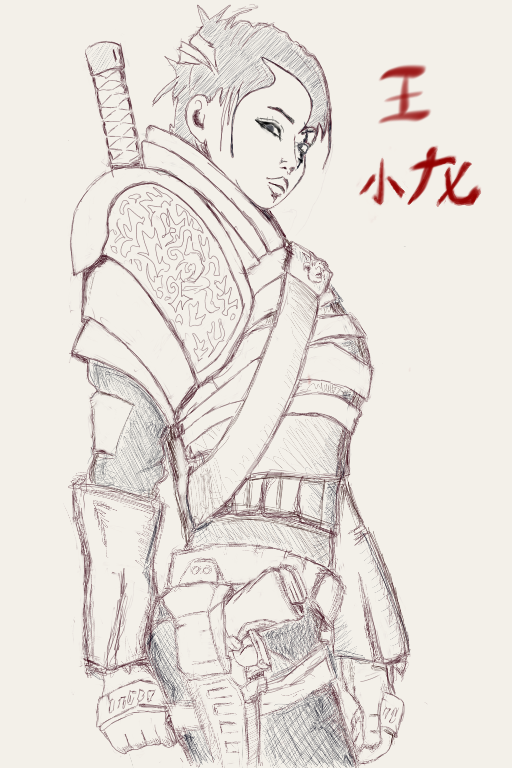
\includegraphics[width=0.9\linewidth]{./images/wang_xiao_long.png}}
    \caption{\xl}
\end{wrapfigure}

Vor zwei Jahren geriet \xl{} auf Callisto nach einem Zusammensto\3 mit der Sun Ye On Sekte in Gefangenschaft und wurde vom Konzerngardisten auf Valhalla inhaftiert. Dort unterzog man sie unter gro\3er Geheimhaltung einem klinischen Eingriff. Bei diesem Eingriff wurde der von Prof.~Dr.~Naratova entwickelten ``freien KI'' Symbiont in ihrem Gehirn frei gesetzt. Die Oeration wurde durch Prof.~Dr.~Sanders durchgef"uhrt. Prof.~Dr.~Sanders handelte dabei im direkten Auftrag von Prof.~Dr.~Naratovas ohne das Wissen der USI Agenten. Durch ihre starke Pers"onlichkeit konnte \xl{} verhindern da\3 die KI ihren Geist vollst"andig "ubernehmen konnte und so verschmolzen der Geist und das artifizielle Gehirnzu einer Symbiose genau so wie Prof.~Dr.~Naratova es sich immer erhofft hatte. Der neu entstandene KI--Mensch Twitter wurde nach einem vorget"auschten Hirntod aus der Haftanstalt geschmuggelt und freigelassen. Nach der ersten Regenration in einem Schmuggellager schlo\3 sie sich \xl{} dem Luna--Syndikats an um auf Valhalla Nachforschungen zu ihrer ungewollten Verwandlung anzustelle. Als Pirat und Schmugglerk"onig wohlbekannt fand sie bei Nemessis einen wilkommenen G"onner. Die Verwandlung in eine KI ist au\3er Ihr, Naratova und deren Mitarbeitern niemandem bekannt.

\xl{} ist eine hochgewachsene Asiatin Anfang 40, ein Pure, die sich als Samurai mit entsprechender R"usting pr"asentiert. Sie ist intelligent, gewitzt, skrupellos und liebt das Risiko. Durch ihre finanziellen M"oglichkeiten und Kontakte in ihrem fr"uheren Leben hat Sie ihren K"orper durch zahllose Modifikationen zu einer Kampfmaschiene entwickelt die einem Omega in nichts nachsteht.

Im Rahmen des Abenteuers verfolgt sie das Ziel die Forschungsergebnisse Naratovas an sich zu bringen und alle Informationen zu den freien KIs wie auch das Wissen "uber die Technologie zu vernichten. Daf"ur wird sie alle an den Experimenten beteiligten Personen, Naratova, Sanders, die USI Agenten und deren Wissenschaftler t"oten und Forschungseinrichtungen zerst"oren solange sie dabei den Verdacht nicht zu offensichtlich auf sich lenkt. An der Identit"at der anderen KIs ist sie nicht interessiert. Im Umgang mit den anderen  Gangstern des Luna Syndikats tritt sie als Anf"uhrerin auf.

Vor dem Zusammentreffen mit den Charakteren kennt sie den Standort und den Namen der USI Tochter Cyberbrain nicht.

\pinyin{Wang2} \pinyin{Xiao3} \pinyin{Long2}: Fight +9, Agility +10, Body +4, HP 14

\section{Carina alias Fleur Soleil}

\begin{wrapfigure}{r}
    {0.50\textwidth}\fbox{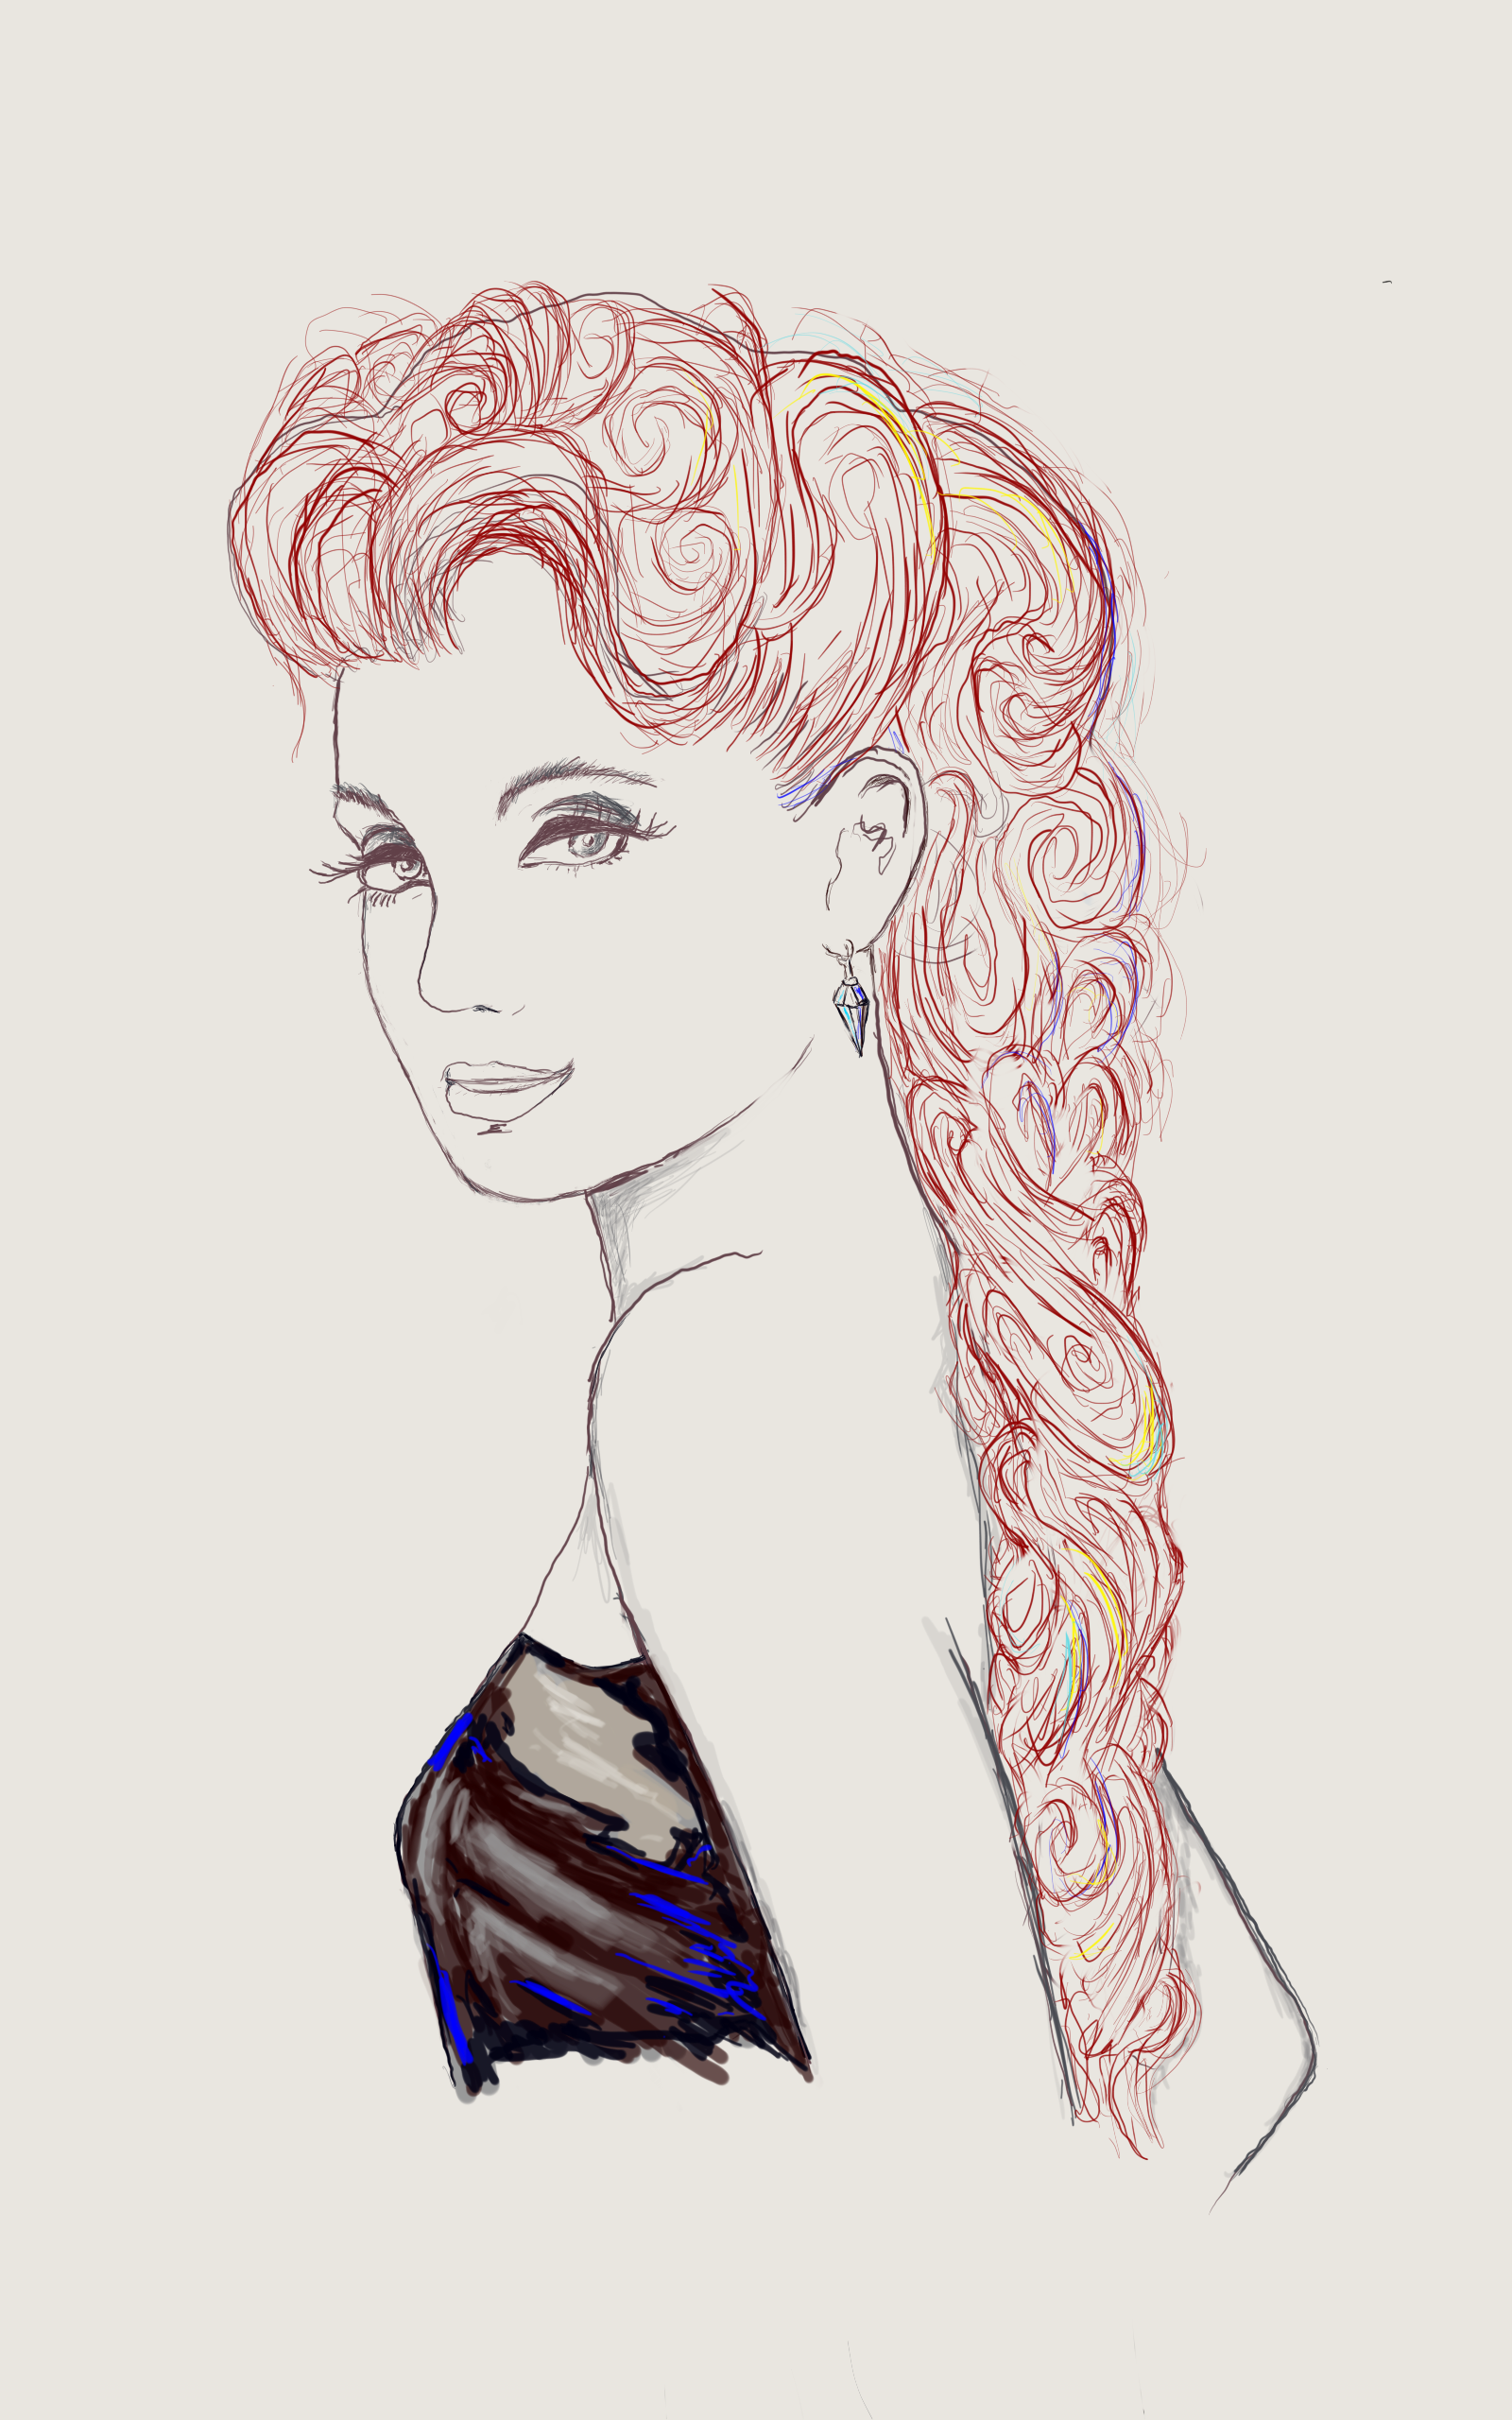
\includegraphics[width=0.9\linewidth]{./images/carina.png}}
    \caption{Carina}
\end{wrapfigure}

Die als geheimnisvolle Freundin von Slingshot erstmals aufgetauchte Frau mit auff"alligen roten Haaren ist im Blackhole Club als Carina bekannt und stellt dort Kontakte zwischen Anbietern und Interesenten von Waren und Dienstleistungen her. Sie arbeitet dabei mit dem Barmann Rosen zusammen. Im Ice Club tritt sie unter dem Namen Fleur Soleil als S"angerin und f"ur ausgew"ahlte Kundschaft auch f"ur andere Dienste auf. Carina ist sehr h"ubsch, vielleicht Ende 20 und lebenslustig. Ihr auff"alligstes Merkmal und Markenzeichen sind lange kunstvoll geflochtene Haare. Die Farbe der Haare kann sie je nach Stimmung und Gelegenheit in nahezu beliebige Farben wechseln.

Carina hat den Erstkontakt von Hanibal und Slingshot zu den USI Agenten Smith--Singer und Frederic Johnson hergestellt. Mit Slingshot war sie f"ur kurze Zeit n"aher befreundet und ist entsprechend von seinem Tod und ihrer Mitt"aterschaft ersch"uttert und will den Ermittlern 
aus diesem Grund auch weiterhelfen.

\section{Nemessis}

Nemessis ist der Duke von Valhalla, der Pate des Luna--Syndikats. Nemessis ist ein Slag dessen K"orper sich nicht mehr selbst am Leben erhalten kann. 

\begin{wrapfigure}{r}
    {0.70\textwidth}\fbox{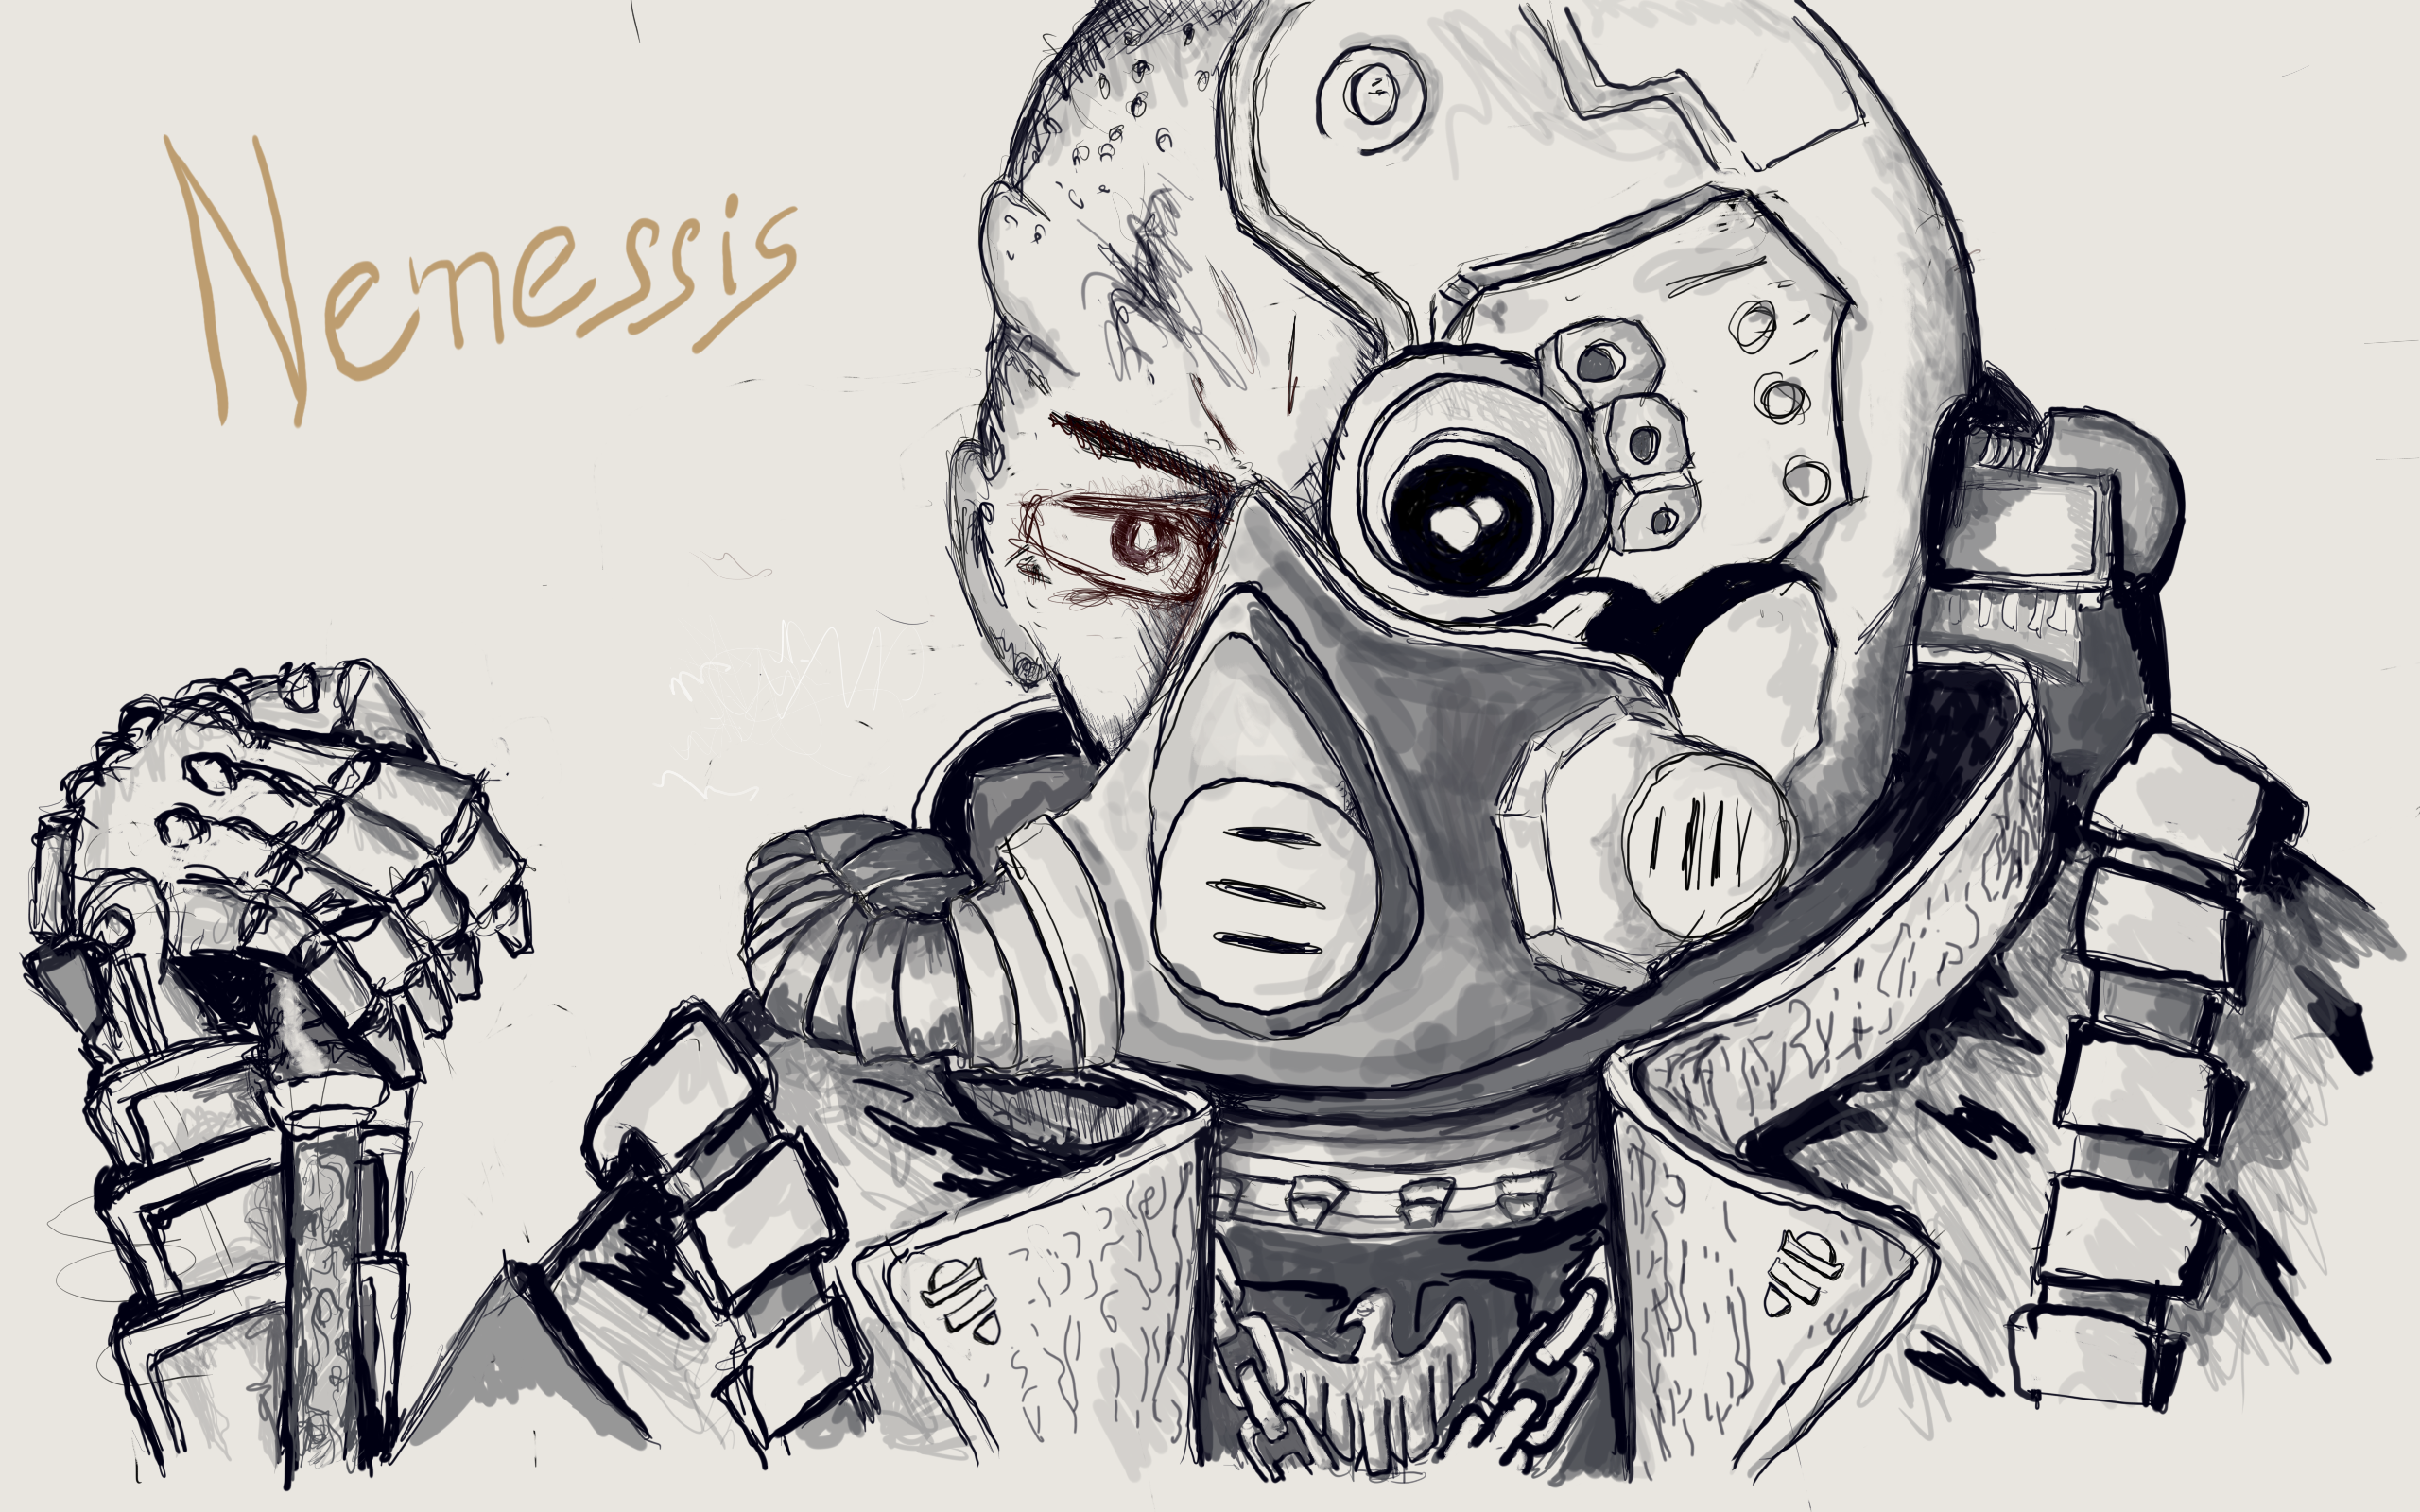
\includegraphics[width=0.9\linewidth]{./images/nemessis.png}}
    \caption{Nemessis}
\end{wrapfigure}

Ein Gro\3teil seiner Gliedma\3en und sonstigen K"orperfunktionen sind durch synthetische Teile ersetzt die Ihm das Aussehen eines Cyborgs geben. Nemessis hat die Unterwelt auf Valhalla durch seine gut organisierten Untergebenen und sein weitreichendes Kontaktenetz
fest im Griff. Das Syndikat betreibt das lokake Fusionskraftwerk von Valhalla und damit die Lebensversorung. Ein Gro\3teil der Etablisments in Paradise City werden vom Luna Syndikat betrieben. Nemessis hat mit Blackheart die Vereinbarung getroffen da\3 sich die Protektoratsstreitkr"afte nicht in seine Aktivit"aten einmischen er daf"ur den reibungslosen Betrieb Valhallas sicherstellt.


\newpage
\section{USI Agenten}

Die United Space Industry (USI) finanziert das KI Projekt, betreibt "uber Stohfirmen die Cyberbrain Forschungseinrichtung auf Kallisto und beauftragt die Attent"ater. Vor Ort im jovianischen System koordiniert der Agent \emph{J.~Smith--Singer} die Operation P9. Smith--Singer wird druch den Psychonauten \emph{Frederic Johnson}, den Strohmann \emph{Dan Ringdaz} und die beiden S"oldner \emph{Lazor} und \emph{Flinn}. Den Erstkontakt zu Prof.~Dr.~Naratove stellte ein Agent her den der Ermittlercharakter als Prolog Interviewen durfte.

Smith--Singer gibt sich als Agent des Konzernrat aus und hat auch die M"oglichkeiten in gewissem Rahmen als dieser zu agieren. Vor dem Eintreffen der Charaktere auf Valhalla treten die USI Agenten nicht in Aktion. Die Agenten setzen sich auf Valhalla nach der Landung der Dawn--of-Day an die Fersen. Die Identit"at der Charaktere kann aber je nach Spielverlauf bis zur \emph{"`Im Ice Club"'} Szene zur"uck gehalten werden. Die USI Agenten kennen die agierenden Mitglieder des Luna Syndikats nicht und wissen nichts von den freien KIs.

Ziel der USI Agenten ist es:

\begin{itemize}
    \item Nach der Willkommensgala: Sicherstellen der Forschungsergebnisse von Prof.Dr.~Naratova
    \item Informationen "uber die Forschung und die Identit"at der Attent"ater so lange wie möglich zu vertuschen.    
\end{itemize}

Der prim"are Gegenspieler der Ermittler ist J.~Smith--Singer. Smith Singer ist ein Pure mit der Statur eines Bodyguards. Sein Name wird in verschiedenen Situationen erw"ahnt.

\begin{itemize}
    \item Smith--Singer \\
          Fight +7, Agility +7, Body + 3, Communicaion +7 HP 12
    \item Frederic Johnson\\
          Fight +3, Agility +4, Body +2 Communication +6 Psychonaut +6 HP 10
    \item Dan Ringdaz\\
          Fight +4, Agility +4, Body +1, Communication +6 HP 10
    \item Lazor\\
          Fight +6, Agility +5,  Body +2, HP 12
    \item Flinn\\
          Fight +6, Agility +5,  Body +2, HP 12
    \item Schl"ager\\
          Fight +2, Agility +1, Body +1, HP 10
\end{itemize}

\section{Technischer Betrieb der Zone}

Der technische Betrieb und die Wartung der Zone erfolgt durch das Unternehmen Dockbunner das Norms und Alpha Mutanten 
besch"aftigt.

Dockbunner Mitarbeiter Fight +2, Agility +2, Technics +5, HP 10

\section{Sicherheitsgardisten die Zone}

Um die Sicherheit der Einrichtungen der sog.~Zone auf Valhalla ist das Unternehmen TransSec zust"andig. TransSec stellt
Wachpersonal in Form von Norm Sicherheitskr"aften zur Verf"ugung die die G"ange der Zone patroullieren. Die Sicherheit
innerhalb der Geb"aude "ubernehmen die jeweiligen Unternehmen selbst.

Konzerngardist Fight +3, Agility +3, Body +1, HP 10, Bodyarmor -6, Railgun +5, Boltgun +3

\section{Sto"strupp Cynarion}

Zur Unterst"utzung der Charaktere zur die Infiltration der Cyberbrain Forschungseinrichtung kann Cynarion bis zu 
drei S"oldner bereit stellen.

\begin{itemize}
    \item Lionel Badger: Fight +5, Agility +3, Body +1, HP 12, Bodyarmor -6
    \item John Bozo: Fight +5, Agility +3, Body +1, HP 12, Bodyarmor -6
    \item Flint Ross (Sicherheitsspezialist): Fight +2, Agility +2, Body +1, Technics +5, HP 10, Bodyarmor -6
\end{itemize}

Bewaffnung: Railgun +5, Boltgun +3, Vibro Klinge +2, Granate +6, Schockgranate/EMP +6 

\section{Sto"strupp Protektoratsgarnison}

Zur Unterst"utzung der Charaktere zur Infiltration  Cyberbrain Forschungseinrichtung kann die Protektoratsarmee eine 
Omega Special Ops Gruppe bereit stellen.

\begin{itemize}
    \item Stormball (Truppf"uhrer): Fight +7, Agility +7, Body +5, HP 12, Bodyarmor -6
    \item Thunder (Attent"ater): Fight +7, Agility +7, Body +5, HP 12, Bodyarmor -6
    \item Jackhammer (Sicherheitsspezialist): Fight +6, Agility +6, Body +5, Technics +5, HP 12, Bodyarmor -6
\end{itemize}

Bewaffnung: Railgun +5, Boltgun +3, Vibro Klinge +2, Granate +6, Schockgranate/EMP +6 

Bei Thunder handelt es sich um einen durch eine KI infiltrierten Attent"ater der bei Zusammentreffen mit den 
Mitarbeitern des Forschungsinstitutes einen Angriff durchf"uhrt.

\renewcommand{\ml}{\pinyin{Mailin2}}

\section{Mitarbeiter Cyberbrain}

Cyberbrain ist das Forschungsinstitut in dem die ersten Attent"ater operiert wurden. Mit der Aufl"osung der Forschungsstation von Seite Neurointelligence befinden sind betraut:

\begin{itemize}
    \item Dr.~Dan Leitner: Technischer Projektleiter. Mitarbieter bei der Etnwicklung der Nanobots. Spezialist f"ur die Verschmelzung 
        der  Nanobots mit den Neuronen des Gehirns.
    \item \ml{}: Programmiererin. Erschaffering der freien KIs. Eine kleine Taiwanesin Anfang 30. 
    \item Dr.~Gaius Ross: Techniker f"ur medizinische Ger"atschaften. Spezialist f"ur die Commandchip. Steuewrung der Nanobots.
    \item Francis McDonald: Systemadministrator.
\end{itemize}

\newpage
\section[Mailin]{\ml{}}

\ml{} ist eine Mitarbeiterin von Prof.~Dr.~Naratova. Auf Nike ist sie die Hauptprogrammiererin die die KI Software der USI auf den Einsatz in einem menschlichen Gehirn angepasst hat.  In der Cyberbrain Forschungseinrichtung hat sie die KIs auf ihre Tr"ager kalibriert.

\begin{wrapfigure}{r}
    {0.6\textwidth}\fbox{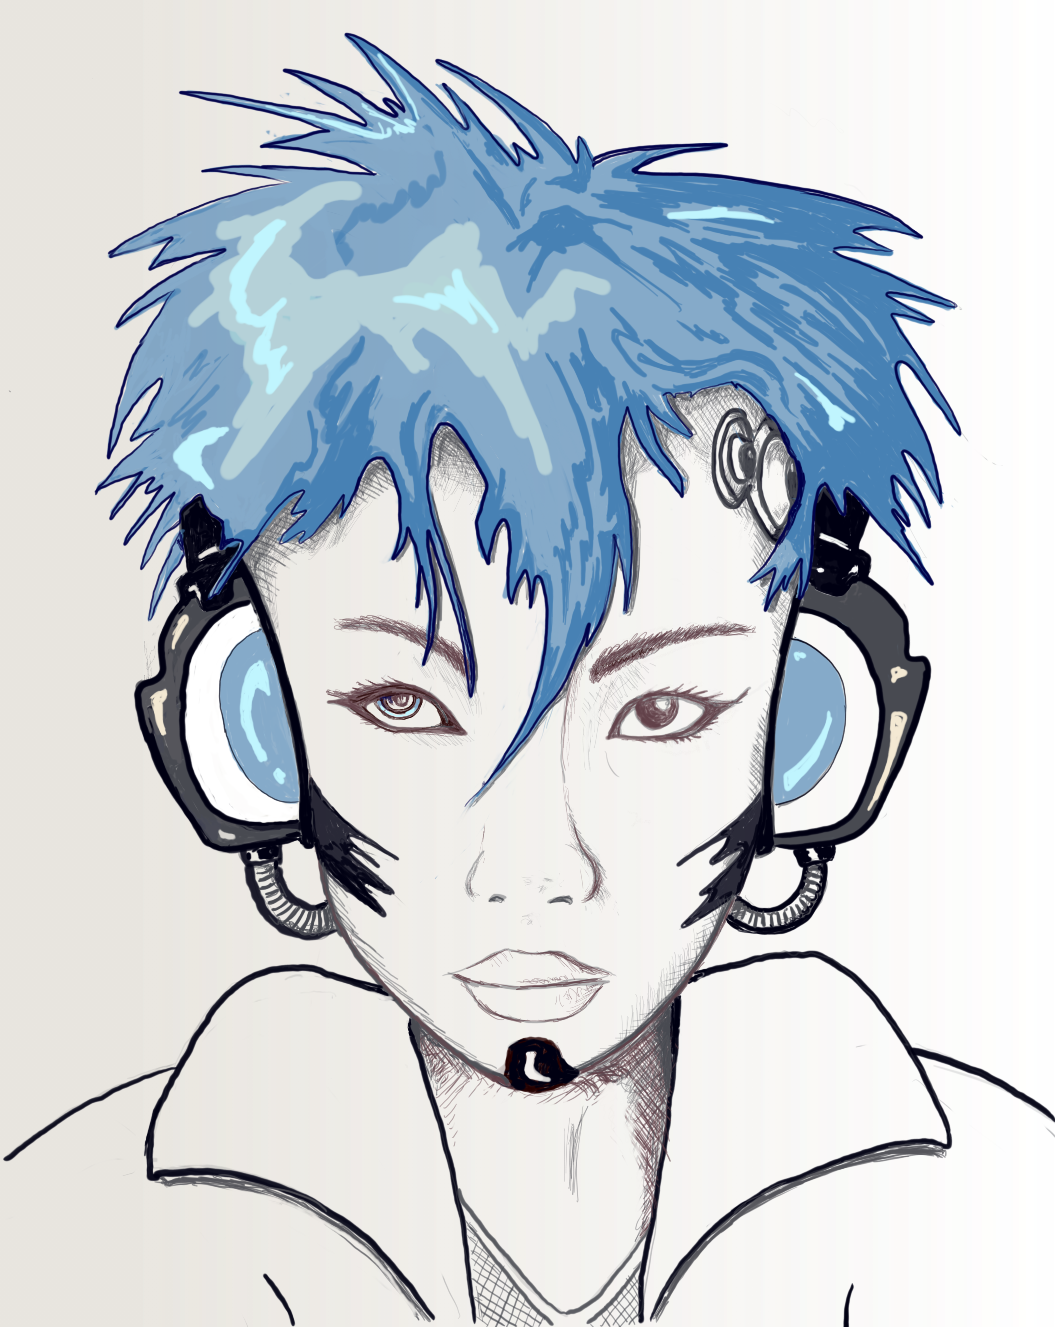
\includegraphics[width=0.9\linewidth]{./images/mailin_final.png}}
    \caption{\ml{}}
\end{wrapfigure}

Nach der Entdeckung da\3 die KIs mit einer Routine zur Bindung an die USI versehen wurde hat sie in geheimer Absprache mit Prof.~Dr.~Naratova eine modifizierte Version der KI entwickelt die die KIs von den Zw"angen der USI befreiten. Gleichzeitig modifizierte sie aber den Code so, da\3 die freien KIs sie und Prof.~Dr.~Naratova nicht angreifen k"onnen und sie zu besch"utzen versuchen w"urden. Ihr pers"onliches Ziel ist es unbeschadet aus der aktuellen Konfliktsituation und wie Dr.~Naratove die Forschungen an den KIs weiter zu betreiben. Im Kep"ack hat sie den Code der von ihr geschaffenen Generation der freien KIs.

\ml{} ist klein, h"ubsch und hat einen verschlagenen Zug. Im Gespr"ach arbeitet sie gerne mit Andeutungen und Umschreibungen.

\section{Guardian Klasse Schlachtkreuzer}

Bei den Guardian Klasse Schlachtkreuzern mit der Bezeichnung Zeus II-1 und Zeus II-2 handelt es sich um KI gesteuerte Gro\3kampfschiffe aus den Iridium Kriegen. Nach ihrer "Achtung traten sie das erste mal wieder beim Kampf der Mutanten gegen die Europ"asche F"orderation im erdnahmen Orbit auf und verschwanden danach auch wieder wie sie gekomme waren.

Die Guardian Kreuzer besitzen gegen"uber den "ublichen Kreuzern viel weniger Platz f"ur Personen sind aber daf"ur aber mit einem gr"o\3eren Jagdgeschwader "ahnlich einem Flottentr"ager ausgestattet. Ein Guardian Schlachktreuzer beherbergt zwei Staffeln von KI gesteuerten J"agern, eine Kompanie KI Kampfdrohnen und 15 Landungsschiffen.

Die KI Kampdrohnen sind spinnenartige Roboter ausgestattet mit zwei schweren vollautomatischen Railguns, Schwei\3ger"aten und einer kleinen Plasmaschleuder.

Fight +8, Agilty +6, Body +6, HP 15, Panzerung -6

